\chapter{Proposta de Extensões ao Modelo NCM e à Linguagem NCL} \label{cap:cap4}

A Linguagem NCL \textit{Nested Context Language}) é baseada no modelo conceitual NCM (\textit{Nested Context Model}). Esta tese propõe extensões ao modelo NCM e à linguagem NCL para incluir as facilidades de interação multimodal e suporte multiusuário. As próximas seções detalham as extensões propostas.

\section{Extensões ao Modelo NCM}
\label{sec:NCMExt}

A extensão ao Modelo NCM (\textit{Nested Context Model}) proposta nesta tese se divide em duas partes. A primeira parte diz respeito a novas entidades NCM para suporte a múltiplos usuários, proposta que estende as ideias de \cite{guedes2016extending}, e também informações de contexto, considerando a abordagem apresentada em \cite{Josue:2018:MSE:3204949.3204967}. A segunda  parte diz respeito à criação de novos tipos de eventos no modelo NCM para dar suporte à interação multimodal, propondo uma abordagem diferente da proposta de \cite{guedes2016extending}. 

\subsection{Multiusuário}
\label{sec:MultUser}

Em relação à modelagem dos usuários que participam de uma experiência multimídia, diferente de \cite{guedes2016extending}, este trabalho representa um usuário individualmente com suas características específicas que poderiam, por exemplo, ser carregadas de um perfil especificado em uma arquivo XML no padrão MPEG-21 parte 22 \cite{ISO/IEC:2019aa}. As características podem conter desde preferências de tipos de mídia até limiares de percepções como volume de som, luminosidade, etc. 

Para representar os usuários individualmente de maneira especifica é proposta a entidade  \textit{userAgent}. Um \textit{userAgent} indica um único usuário e tem o atributo \textit{src}, que indica a especificação de suas características específicas. 

%Neste caso existe associação de uma instância da classe \textit{UserSettingsNode} para cada usuário armazanando as propriedades carregadas do arquivo XML. 

Para representar um perfil de usuário, foi proposta a entidade \textit{userProfile}, que contém o atributo \textit{src} para indicar as características do perfil de usuário em questão. 

Para que as características de um usuário específico ou de um perfil possam ser usadas em elos entre nós de um documento NCM, é proposta a entidade \textit{UserSettingsNode}, que faz referência a um usuário (\textit{userAgent}) ou perfil (\textit{userProfile}), permitindo o uso de eventos de atribuição relacionados a propriedades desse nó. A Figura \ref{fig:exNCM_MultiUsuario} ilustra tais entidades.

\begin{figure}[h!]
    \centering
    \begin{tikzpicture}
        \umlclass[fill=orange!40]{UserAgent}{ - src}{}
        \umlsimpleclass[y=-3, fill=orange!40]{UserSettingsNode}{}{}
        \umlclass[x=5, fill=orange!40]{UserProfile}
             {- src \\- max \\- min}{}
        \umlassoc[mult1=1, mult2=1]{UserAgent}{UserSettingsNode}
    \end{tikzpicture}
    \caption{Entidades para suporte multiusuário}
    \label{fig:exNCM_MultiUsuario}
\end{figure}

\subsection{Informação Contextual} \label{sec:InfCont}

%Em NCM, eventos são associados a máquinas de estado. Considerando nós de conteúdo, tais máquinas de estado podem caracterizar eventos de \textbf{apresentação} (apresentação do conteúdo associado ao nó), eventos de  \textbf{atribuição} (mudança de valores de seus atributos) ou eventos de \textbf{interação multimodal}, como será discutido mais adiante no texto. 

%Analisando a extensão proposta em \cite{josue2018preparation}, objetos de mídia cujo conteúdo é obtido através da rede, podem levar um certo tempo para ser carregado pelo \textit{player}, e em alguns casos gerar falhas de sincronização na apresentação da aplicação multimídia. Visando reduzir atrasos na apresentação desses objetos de mídia, os autores de  \cite{josue2018preparation} propõem estender a linguagem NCL, através da incorporação do evento de preparação. O evento de \textbf{preparação} pode ser definido sobre um objeto de mídia, para representar o carregamento antecipado do conteúdo da mídia e a instanciação do \textit{player} responsável pela sua reprodução. Este tempo, portanto, seria representado pela duração do evento de preparação. O evento de preparação entra no estado \textit{occurring} uma vez que os \textit{players} são ativados e volta para o estado \textit{sleeping}, quando sua execução termina. O evento de preparação está relacionado com o de apresentação, de forma que quando o evento de preparação termina, o evento de apresentação está apto para iniciar.

No modelo NCM, a entidade \textit{SettingsNode} é do tipo \textit{ContentNode}, portanto herda todas as características especificadas em nó de conteúdo como por exemplo suas propriedades. %Desta forma, usar uma entidade deste tipo proporciona recorrer à máquina de estados dos eventos relacionadas a suas instâncias e assim referenciarmos os eventos por meio dos elos do NCM e ter o acionamento de ações. 
Esta tese propõe que a representação de informações contextuais tanto de ambiente como de usuário sejam modeladas como um subtipo de \textit{SettingsNode}.  %conjunto de atributos (propriedades) de nós representando características do usuário e do ambiente. 
A Figura~\ref{fig:node_settings} ilustra os dois tipos específicos de nó, \textit{AmbientSettingsNode} e \textit{UserSettingsNode}, ambos subtipos do nó \textit{SettingsNode} de NCM. Na figura, uma lista de atributos reduzida é apresentada para exemplificar diferentes características de usuários e ambientes que podem ser modeladas. Na entidade \textit{UserSettingsNode}, o atributo \textit{heartbeat} contém o batimento cardíaco de um usuário específico, \textit{temperature} a sua temperatura corporal, e o \textit{age} sua idade. Já o atributo \textit{user}, que relaciona esta entidade à entidade \textit{UserAgent}, identifica o usuário diante dos outros como foi descrito na Seção~\ref{sec:MultUser}. Desta forma, possibilita-se carregar todas as características  associadas ao \textit{UserAgent} no nó \textit{UserSettingsNode} correspondente, assim suas informações individuais estarão acessíveis por meio de um nó de conteúdo. É importante ressaltar que outros atributos podem ser adicionados às entidades \textit{AmbientSettingsNode} e \textit{UserSettingsNode}, além do fato de que um documento NCM pode conter mais de uma instância dessas entidades, diferente de como acontece com \textit{SettingsNode}, que só pode conter uma ocorrência por documento na especificação de NCL 3.0. 

\begin{figure}[h!]
\centering
\begin{tikzpicture}
\umlclass{SettingsNode}{}{}
\umlclass[x=-3,y=-3,fill=orange!40]{AmbientSettingsNode}
        {- temperature \\ - luminosity \\ - area \\- ... }{}
\umlclass[x=3,y=-3,fill=orange!40]{UserSettingsNode}
        {- heartbeat \\ - temperature \\- age \\- user \\- ...  }{}

\umlinherit[geometry=-|]{AmbientSettingsNode}{SettingsNode}
\umlinherit[geometry=-|]{UserSettingsNode}{SettingsNode}
\end{tikzpicture}
\caption{Nós para representação de características de usuários e de ambientes}
\label{fig:node_settings}
\end{figure}

É importante notar que os nós apresentados na Figura~\ref{fig:node_settings} são capazes de armazenar informações coletadas por sensores presentes na instalação física (e.g. temperatura, luminosidade, umidade, etc) ou ligados ao usuário (e.g. batimento cardíaco, pressão sanguínea, etc.). Essa é uma abordagem que permite ao autor da aplicação considerar o estado do ambiente ou do usuário para a definição do comportamento da aplicação ou sua adaptação.

\subsection{Interação Multimodal}
\label{sec:MulModal}

O suporte à interação multimodal pode trazer uma sobrecarga a mais para a autoria de aplicações multimídia. Assim, seria ideal que autores que desenvolvem essas aplicações multimídia não se preocupem com detalhes sobre a implementação da captação da interação ou a definição de outras linguagens específicas como SRGS (\textit{Speech Recognition Grammar Specification}), como ocorre na proposta de \cite{Guedes:2016aa}. A integração de novos tipos de interação em sistemas multimídia, além das modalidades tradicionais por mouse e teclado, é um tema abordado em diferentes propostas na literatura \cite{de2011multimodal,nery2008desenvolvimento, batista2010estendendo}. De acordo com Lima et al. \cite{de2011multimodal}, o uso da linguagem natural juntamente com o gesto pode superar as limitações da interação de apenas uma modalidade. Isto porque a combinação de fala e gesto fornece um comportamento comunicativo altamente eficiente para interagir com aplicativos em uma experiência mais transparente que as interfaces tradicionais. 

Sistemas com interação multimodal podem ser classificados de várias formas, dependendo se há fusão dos dados de mais de uma modalidade e se o uso de modalidades é em sequencial ou em paralelo. Em Turk et al. \cite{turk2014multimodal}, há uma discussão aprofundada sobre a classificação de sistemas multimodais. Em um sistema multimodal exclusivo, as modalidades são usadas sequencialmente e estão disponíveis separadamente, mas não integradas pelo sistema. Em um sistema multimodal alternativo, as modalidades são usadas sequencialmente, mas são integradas em algum grau. Em um sistema multimodal concorrente, as informações modais estão disponíveis em paralelo, mas separadamente (não integradas). Finalmente, em um sistema multimodal sinérgico, os modos estão disponíveis em paralelo e totalmente integrados. 

Em geral, os sistemas multimodais disponíveis comercialmente não incluem o processamento paralelo de múltiplos modos de entrada e não utilizam uma fusão destes dados, mas, em vez disso, processam apenas uma alternativa de modo por vez \cite{furht2008encyclopedia}. Neste trabalho, também consideramos as modalidades sendo disparadas uma da cada vez, sendo assim chamado de sistema multimodal exclusivo, de acordo com a classificação apresentada em Turk et al. \cite{turk2014multimodal}.

O modelo NCM já prevê diversos eventos relacionados com a interação do usuário e também atributos que são alterados com a ocorrência destes eventos. Conforme~\cite{Soares:2005qy}, os eventos podem ser dos seguintes tipos: apresentação, composição, seleção, superposição, arraste, foco e atribuição. A evolução tecnológica possibilita a exploração de outras modalidades de interação como reconhecimento de gestos ou voz. Para isso, este trabalho propõe novos tipos de eventos NCM. Por exemplo, dispositivos que mapeiam o movimento dos olhos podem ser utilizados para disparar o evento \textit{eyeGaze}. Portanto, esta tesse propõe outros eventos de interação do usuário, além do evento de seleção, tais como: \textit{touch}, \textit{motion}, \textit{eyeGaze}, \textit{pointer}, \textit{voiceRecognition}, \textit{gestureRecognition}, \textit{handPoseRecognition} ou \textit{faceRecognition}. Eles representam respectivamente a interação por toque, movimento do corpo, fixação do olhar, apontamento, reconhecimento de voz, reconhecimento de gesto, reconhecimento de pose da mão e reconhecimento de expressão facial.  

Tais eventos possuem atributos específicos que especializam o evento. Assim como o atributo \textit{key} indica a tecla que foi selecionada em um evento de seleção, esse atributo é usado de forma similar pelos outros tipos de evento. Por exemplo, para um evento de \textit{gestureRecognition}, o \textit{key} igual a \textit{handUp} indica a ocorrência de um gesto de levantar a mão. A definição da semântica dos valores de tal atributo, ou seja, dos tipos de gestos, comandos de voz, expressões faciais, etc., é dependente do tipo de evento em questão. A Figura~\ref{fig:NCMExt} mostra os tipos de evento propostos por esta tese e a Tabela~\ref{tab:eventos} descreve cada um deles.

\begin{table}[h!]
\centering
\caption{Novos eventos de interação propostos para NCM}
\label{tab:eventos}

\begin{tabular}{ m{5cm} | m{7cm} }
    Nome de Evento & Descrição do tipo de interação\\ \hline
    \textit{touch} & interação por toque\\\hline
    \textit{motion} & movimento do corpo\\\hline
    \textit{eyeGaze} & fixação dos olhos\\\hline
    \textit{pointer} & apontamento\\\hline
    \textit{voiceRecognition} & reconhecimento de voz\\\hline
    \textit{gestureRecognition} & reconhecimento de gesto\\\hline
    \textit{faceRecognition} & reconhecimento de expressão facial\\\hline
\end{tabular}
\end{table}

Uma vez definidos diferentes usuários na aplicação, o autor pode definir relacionamentos com eventos que ocorram somente quando determinados perfis de usuário (ou um usuário específico) realizam uma ação. Para permitir essa nova funcionalidade, os eventos e conectores NCM foram estendidos também. Um evento de interação possui, além de seus atributos definidos por NCM, um atributo \textit{user} que identifica o usuário que disparou o evento durante a execução da aplicação. Seguindo a abordagem de \cite{Guedes:2016aa}, conectores, mais especificamente suas condições, também possuem um atributo adicional \textit{owner}, permitindo a identificação do perfil do usuário na condição de uma relação causal. Quando da execução da aplicação, o reconhecimento ou validação do usuário poderá ser feito de várias maneiras: usando identificação por RFID~\cite{want2006introduction}, reconhecimento facial, \textit{scanner} ou até mesmo temperatura corporal. 

%\begin{landscape}
\begin{figure}
    \centering
    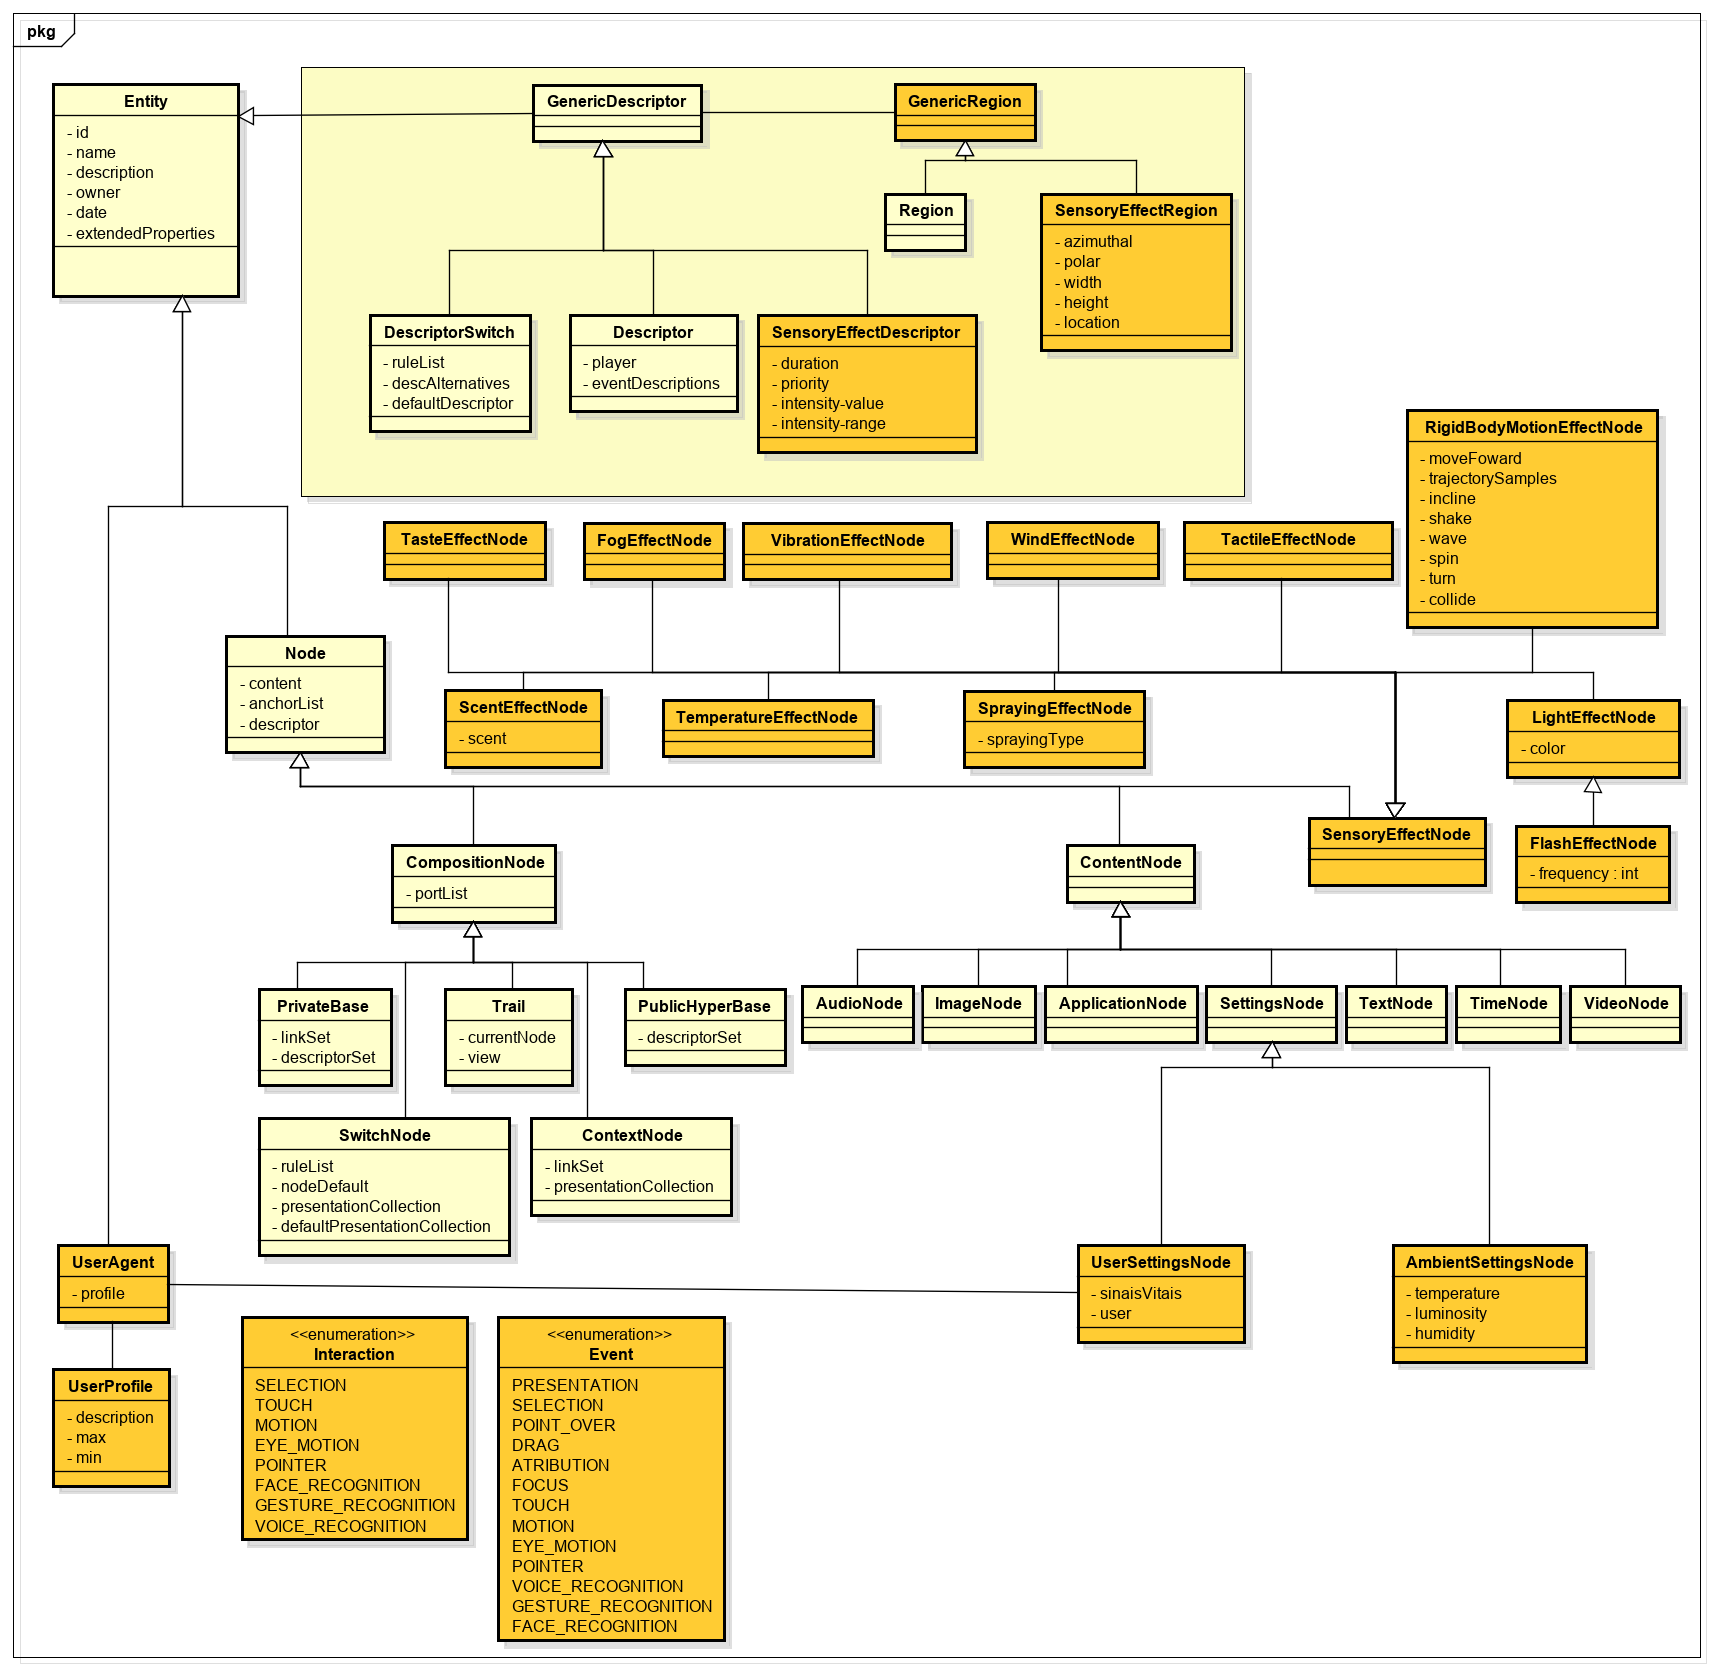
\includegraphics[scale=0.35,keepaspectratio=true]{figuras/NCM.png}
    \caption{Modelo NCM estendido.}
    \label{fig:NCMExt}
\end{figure}
%\end{landscape}

A Figura~\ref{fig:NCMExt}  apresenta o modelo NCM estendido conforme as propostas desta tese. As cores da figura ajudam a identificar o escopo deste trabalho. As entidades em amarelo fazem parte do modelo NCM 3.0 já existente. As entidades de cor laranja estão sendo propostas por este trabalho. Pode-se observar as entidades \textit{UserSettingsNode} e \textit{AmbientSettingsNode} como subclasses da entidade \textit{SettingsNode}, portanto herdando todas suas características como foi dito anteriormente. Pode-se observar também as entidades \textit{UserAgent} e \textit{UserProfile}, ambas subclasses de \textit{Entity}, \textit{UserAgent} associada com \textit{UserProfile} e \textit{UserSettingsNode}. A cardinalidade da associação de \textit{UserAgent} com \textit{UserProfile} é de muitos pra muitos pois um usuário pode ter vários perfis como por exemplo ter um perfil de esportista e ser um professor. Desta forma, o nó de conteúdo (\textit{UserSettingsNode}) que armazena as informações desse usuário pode armazenar informações desses dois perfis. E obviamente um perfil pode estar associados a vários usuários. Já a associação de \textit{UserAgent} com \textit{UserSettingsNode} é de um pra um. A Figura~\ref{fig:NCMExt} inclui também as entidades relacionadas a efeitos sensoriais, que foram propostas em Josue et al.\cite{Josue:2018:MSE:3204949.3204967}.

Além da extensão do modelo NCM, apresentada na Figura~\ref{fig:NCMExt}, este trabalho propõe uma extensão da linguagem NCL de maneira que o autor consiga usar novas facilidades para representação de múltiplos usuários e diferentes eventos de interação em sua aplicação multimídia. A extensão da linguagem NCL é discutida na próxima seção.

\section{NCL 4.0}

Para implementar as alterações no modelo NCM descritas na Seção~\ref{sec:NCMExt}, esta tese e os trabalhos \cite{barreto2019authoring,montevecchi2020providing,valentim2020possibilitando,Josue:2018:MSE:3204949.3204967, barreto2019ncl_u, barreto2019providing_MU,barreto2019providing} propõem uma extensão da linguagem NCL (\textit{Nested Context Language}) denominada NCL 4.0. Diversas alterações são sugeridas para expressar as entidades idealizadas na extensão do modelo proposta neste trabalho. A proposta de NCL 4.0 
é especificada utilizando \textit{XML schema} \cite{thompson2004xml}. O esquema proposto foi estendido do esquema da linguagem NCL 3.0\footnote{http://www.ncl.org.br/pt-br/schemasxml}. A extensão proposta contém os novos elementos além de alterações nos elementos existentes para contemplar o que foi modelado\footnote{https://github.com/FabioBarr/NCL4.0.git}.

A linguagem NCL 4.0 é divida em módulos e estes são agrupados em área funcionais. 



 
Esta tese foca nas entidades relacionadas com interação multimodal e multiusuário em aplicações multimídia. Para isso, propõe alteração no módulo \textit{Media} da área funcional \textit{Components}, onde foi modificado o elemento \textit{media} acrescentando mais dois tipos possíveis de nós \textit{settings}. Os novos eventos de interação foram contemplados com a alteração do módulo \textit{CausalConnectorFunctionality} da área funcional \textit{Connectors} com adição de novos tipos de evento e também novos papeis de condição predefinidos. Finalmente foi acrescentada uma nova área funcional denominada \textit{Users}, contendo o módulo \textit{User}, que define  os elementos \textit{userAgent} e \textit{userProfile}. 
 
A representação das entidades \textit{UserAgent} e \textit{UserProfile} é feita pela adição dos elementos XML  \textit{<userAgent>} e \textit{<userProfile>}. Tais elementos são definidos para representar um perfil ou um usuário individualmente. O elemento \textit{<userAgent>} possibilita ao autor criar uma aplicação sob medida com a representação de um usuário individualmente. A Tabela~\ref{tab:atUserAgent} apresenta seus atributos. Em \textit{src} é especificado o arquivo XML com as características do usuário seguindo o formato MEPG 21 parte 22 \cite{ISO/IEC:2019aa} e que serão carregadas para o nó \textit{userSettings} correspondente. Desta forma, o autor poderá criar links associados a essas propriedades. Além disso, os eventos de interação pode ser condicionados a usuários especificados com a cláusula <userAgent>.  A Listagem~\ref{lst:userAgent} apresenta um exemplo da definição de um usuário específico em NCL 4.0.

\begin{table}[h]
\caption{Descrição dos atributos do elemento <userAgent>}
\label{tab:atUserAgent}
\centering
{
  % distancia entre a linha e o texto
  \renewcommand\arraystretch{1.25}
  \begin{tabular}{|p{1,5cm}|p{4,5cm}|p{5cm}|p{3cm}|} \hline
   \multicolumn{1}{|c|}{Atributo} & \multicolumn{1}{|c|}{Descrição} & \multicolumn{1}{c|}{Valor} & \multicolumn{1}{c|}{Obrigatoriedade} \\ \hline 
    \textit{id} & Identifica o elemento dentro da aplicação NCL. & Qualquer cadeia de caracteres que comece com uma letra ou um sublinhado ("\_") e que contenha apenas letras, dígitos, "." e "\_". & Obrigatório \\  \hline
    \textit{src} & Define a URI do arquivo com as propriedades do usuário que serão carregadas. & Qualquer cadeia de caracteres que comece com uma letra ou um sublinhado ("\_") e que contenha apenas letras, dígitos, "." e "\_". & Opcional \\  \hline
  \end{tabular}
}
\end{table}

\begin{lstlisting}[language=ncl,label=lst:userAgent, caption={Definição de características de mais de um usuário de perfil diferente participante da aplicação}]
<userBase>
  <userAgent id="userA" src="user1.xml"/>
</userBase>
\end{lstlisting}

Outra maneira de representar os usuários é por meio do elemento \textit{<userProfile>}, da mesma forma que \textit{<userAgent>}, o perfil também tem o atributo \textit{src} que indica o caminho para o arquivo com as propriedades do perfil. Porém, neste caso as propriedades do perfil serão utilizadas para verificar se os usuários encontrado no \textit{setbox} (especificados por arquivos XML, por exemplo) correspondem as propriedades definidas no perfil. Caso haja, as propriedades dos usuários serão carregadas em nós do tipo \textit{userSettingsNode} correspondente. Assim os usuários que atendam ao perfil terão suas  propriedades consideradas pela aplicação. Além disso, para cada link criado com o perfil no parâmetro \textit{user}, serão criados links dinâmicos para todos que atendem o perfil. Tais links terão a identificação do usuário que foi especificada no arquivo de propriedades. A Tabela~\ref{tab:atUserProfile} apresenta os atributos do elemento \textit{<userProfile>} e a Listagem~\ref{lst:userProfile} apresenta um exemplo da definição de um perfil de usuário.  

\begin{table}[h]
\caption{Descrição dos atributos do elemento <userProfile>}
\label{tab:atUserProfile}
\centering
{
  % distancia entre a linha e o texto
  \renewcommand\arraystretch{1.25}
  \begin{tabular}{|p{1,5cm}|p{4,5cm}|p{5cm}|p{3cm}|} \hline
   \multicolumn{1}{|c|}{Atributo} & \multicolumn{1}{|c|}{Descrição} & \multicolumn{1}{c|}{Valor} & \multicolumn{1}{c|}{Obrigatoriedade} \\ \hline 
    \textit{id} & Identifica o elemento dentro da aplicação NCL. & Qualquer cadeia de caracteres que comece com uma letra ou um sublinhado ("\_") e que contenha apenas letras, dígitos, "." e "\_". & Obrigatório \\  \hline
    \textit{src} & Define a URI do arquivo com as propriedades do perfil de usuário. & Qualquer cadeia de caracteres que comece com uma letra ou um sublinhado ("\_") e que contenha apenas letras, dígitos, "." e "\_". & Obrigatório \\  \hline
    \textit{min} & Define o número mínimo de usuários que podem seguir este perfil na aplicação NCL. & número inteiro maior ou igual a zero (valor default é zero) & Opcional \\  \hline
    \textit{max} & Define o número máximo de usuários que podem seguir este perfil na aplicação NCL. & número inteiro maior ou igual ao valor do atributo min ou ``unbounded'' (valor default é ``unbounded'') & Opcional \\  \hline
  \end{tabular}
}
\end{table}


\begin{lstlisting}[language=ncl,label=lst:userProfile, caption={Definição de características de mais de um usuário de perfil diferente participante da aplicação}]
<userBase>
  <userProfile id="profile1" max="1" src="profile1.xml"/>
</userBase>
\end{lstlisting}

E finalmente outra possibilidade de se ter a participação do usuário identificada é sem a utilização do \textit{<userAgent>} e \textit{<userProfile>}. Basta colocar a palavra \textit{"all"} no parâmetro \textit{user} dos links construídos que da mesma forma do perfil, serão criados links dinâmicos para todos os usuários encontrados no \textit{setbox} sem fazer a validação do perfil.  Nós do tipo \textit{userSettingsNode} com valor \textit{"all"} resultarão em criação de nós dinamicamente.

As entidades \textit{UserSettingsNode} e \textit{AmbientSettingsNode} são expressas por meio de modificações no elemento \textit{<media>} onde foram adicionados dois novos tipos, um para representar características do usuário e outro para representar características do ambiente. Tais características podem ser estáticas lidas de arquivos ou dinâmicas lidas de sensores presentes no ambiente e/ou no usuário. Porém a linguagem NCL 3.0 não dá suporte a isso, pois conforme apresentado na norma ABNT NBR15606-2 \cite{ABNT:2011aa}, é permitido o armazenamento de variáveis em NCL 3.0 por meio de um nó <media> do tipo \textit{application/x-ncl-settings}. Estas podem ser globais definidas pelo autor ou de ambiente reservadas para o sistema Ginga. Alguns valores de propriedades do nó do tipo \textit{application/x-ncl-settings} podem ser modificadas através do uso de elos NCL.  Porém, só é permitido um nó do tipo ncl-settings em cada documento NCL. Neste contexto, este trabalho propõe adicionar mais dois tipos de mídia: "\textit{ambient-settings}" e "\textit{user-settings}" que  armazenam informações do ambiente e do usuário respectivamente. Estes com a cardinalidade maior que 1 como os outros tipos de nó \textit{<media>}, além de suas informações poderem ser advindas de sensores que deverão atualizar estes dados periodicamente ou definidos pelo autor do documento NCL. O nó <media> do tipo \textit{ambient-settings} (\textit{application/x-ncl-ambient-settings}) poderá usar a propriedade \textit{descriptor} para especificar um descritor que contém características de leitura das informações dos sensores como por exemplo, frequência de captura. A frequência de leitura indica a cada quanto tempo a mídia será atualizada com dados lidos do sensor.
Um elemento \textit{descriptor} associado a um nó \textit{ambient-settings} pode referenciar o elemento \textit{region} na qual define a região de captura de dados. A maneira com os sensores do ambiente vão ser ligados aos nós de ambiente pode ser definida através de um arquivo de configuração, que será definido no Capítulo~\ref{cap:cap5}.

A Listagem~\ref{lst:ambientSettings} apresenta um exemplo da utilização de \textit{ambient-settings}. O nó com id \textit{propLumRoom} descreve variáveis que irão armazenar características do ambiente, neste caso luminosidade e temperatura. Este nó contém uma propriedade para cada característica.

\begin{lstlisting}[language=ncl,label=lst:ambientSettings, caption={Definição de \textit{AmbientSettingsNode}}]
 <media type="application/x-ncl-ambient-settings" id="propLumRoom" >
   <property name="luminosity" />
   <property name="temperature" />
 </media>
\end{lstlisting}

O nó <media> do tipo \textit{user-settings} (\textit{application/x-ncl-user-settings}) funciona de maneira semelhante ao \textit{ambient-settings}.  A principal diferença é que os sensores não estão associados a um ambiente, mas sim a um usuário especificamente. Além de poder armazenar também características estáticas vindas de arquivos armazenados localmente ou repositórios pré-definidos. Tal arquitetura será definida no Capítulo~\ref{cap:cap5}. Para realizar a associação de sensores a um usuário, deve-se associar a mídia \textit{user-settings} a um \textit{id} de usuário. A Listagem~\ref{lst:ncl_userSettings} apresenta um exemplo da utilização de \textit{user-settings}. Pode ser observado que o \textit{user-settings} do exemplo está associado ao \textit{id} do usuário \textit{userB} definido na Listagem~\ref{lst:ncl_user}. Desta forma, todas as características contidas no XML poderão ser carregadas para o \textit{userSettingsNode} associado a um \textit{userAgent}.

\begin{lstlisting}[language=ncl,label=lst:ncl_userSettings, caption={Definição de \textit{UserSettingsNode}}]
  <media type="application/x-ncl-user-settings" id="propUserB" user="userB">
    <property name="heartBeat" />
    <property name="face" />
  </media>
\end{lstlisting}

Em NCL, utilizando conectores, relacionamentos de interação do usuário podem ser definidos \cite{soares2009programando}. E a definição de um conector é feita por um conjunto de papéis que determinam a função dos participantes da relação. Cada papel descreve um evento associado a um participante da relação. Os eventos de interação possuem o atributo \textit{key} que especifica o que foi reconhecido na interação do usuário. Na linguagem NCL, a interação multimodal é expressa com adição de eventos e novos papéis com os valores possíveis para o atributo \textit{key}. Essa adição de eventos, através dos papeis, segue o que foi modelado no Capítulo XXX representado na Figura~\ref{fig:NCMExt}. Para facilitar o uso desses novos eventos em NCL, são adicionados novos nomes reservados de papéis para o elemento  \textit{<simpleCondition>}. A Tabela~\ref{tab:papModal} apresenta os papeis relacionados a eventos de interatividade multimodal assim como os possíveis valores para o atributo \textit{key} propostos nesta tese.

\begin{table}[h]
\caption{Papeis propostos para contemplar as interações multimodais}
\label{tab:papModal}
\centering
{
  % distancia entre a linha e o texto
  \renewcommand\arraystretch{1.25}
  \begin{tabular}{|p{4,5cm}|p{6,5cm}|p{3,5cm}|} \hline
   \multicolumn{1}{|c|}{Papel} & \multicolumn{1}{|c|}{Descrição} & \multicolumn{1}{c|}{Atributo key}  \\ \hline 
  
    onVoiceRecognition & Quando algo dito pelo usuário for reconhecido enquanto o objeto associado a esse papel estiver sendo apresentado ou com foco. & trecho de voz reconhecido \\  \hline

    onFaceRecognition & Quando alguma expressão facial do usuário for reconhecida enquanto o objeto associado a esse papel estiver sendo apresentado ou com foco. & tipo da expressão facial do usuário \\ \hline

    onHandPoseRecognition & Quando algum gesto feito pelo usuário for reconhecido enquanto o objeto associado a esse papel estiver sendo apresentado ou com foco. & tipo do gesto do usuário \\  \hline

    onEyeGaze & Quando o usuário fixar o olhar em um região enquanto o objeto associado a esse papel estiver sendo apresentado ou com foco. & id do objeto que esta na região "olhada" \\  \hline

    onMotion & Quando algum movimento corporal feito pelo usuário for reconhecido enquanto o objeto associado a esse papel estiver sendo apresentado ou com foco. & tipo do movimento do corpo do usuário \\  \hline
    
    onTouch & Quando alguma interação por toque feita pelo usuário for reconhecida enquanto o objeto associado a esse papel estiver sendo apresentado ou com foco. & tipo do toque  \\  \hline
    
    onPointer & Quando um apontamento realizado pelo usuário for reconhecido enquanto o objeto associado a esse papel estiver sendo apresentado ou com foco. & posição do apontamento \\  \hline

  \end{tabular}
}
\end{table}

Conforme o trabalho de \cite{Josue:2018:MSE:3204949.3204967}, NCL 4.0 contém um novo módulo chamado \textit{Effect} dentro da área funcional \textit{Components}, que define o elemento \textit{effect} e seus atributos. Consequentemente os módulos \textit{Layout} e \textit{Descriptor} foram alterados. Mais especificamente, o \textit{Layout} foi alterado ao acrescentar atributos ao elemento \textit{region} e \textit{Descriptor} foi alterado ao acrescentar atributos ao elemento \textit{descriptor}. As entidades NCM do tipo \textit{SensoryEffectNode} são implementadas através do elemento \textit{<effect>} em NCL 4.0, junto com seus atributos \textit{id}, \textit{type} e \textit{descriptor}. Tais atributos vão identificar, especificar e descrever as características da ocorrência do efeito sensorial. A propriedade \textit{type} será descrita seguindo a nomenclatura de tipos de efeitos sensoriais definidos no padrão MPEG-V \cite{yoon2015mpeg}. Em Josue et al.\cite{Josue:2018:MSE:3204949.3204967}, há uma discussão aprofundada sobre a implementação e descrição de elementos que integram efeitos sensoriais em uma aplicação multimídia imersiva. %E a implementação dos efeitos sensoriais por meio da linguagem NCL 4.0 é descrita em \cite{barreto2019authoring}.


Este capítulo apresentou a propostas de extensão tanto do modelo NCM quanto da linguagem NCL. Essas propostas foram consolidadas em uma nova versão da linguagem NCL, chamada NCL 4.0. Para isso, o capítulo detalhou as novas entidades que fazem parte da extensão assim como as alterações que abrangem o modelo e a linguagem. O capítulo apresentou as duas principais contribuições desta tese em seções que falam sobre multiusuário, informações de contexto e multimodalidade. NCL 4.0 reúne facilidades para especificação de aplicações  multissensoriais interativas e multiusuário, possibilitando a evolução da TV digital interativa para TV imersiva multimodal e multiusuário.

O próximo capítulo apresenta a  implementação de NCL 4.0 no \textit{middleware} Ginga-NCL de todos os elementos propostos assim como alterações necessárias para que o Ginga-NCL contemple a proposta. Desta forma, possibilitando a implementação e a execução de aplicações NCL 4.0 com as funcionalidades citadas.